\chapter{Homework 8 Solutions}
% p449:3,5,7,10,19,21
\begin{problem}[WebAssign, HW8, 1]
  A variable force of $2x^{-2}$ pounds moves an object along a straight
  line when it is $x$ feet from the origin. Calculate the work done in
  moving the object from $x=1$ ft to $x=15$ ft. (Round your answer to two
  decimal places.)
\end{problem}
\begin{proof}[Solution]
Recall the formula for the work done by a fore as a function of distance?
It is given by
\[
W=\int_1^15 F(x)\diff x=
2\int_1^{15} x^{-2}\diff x=
-2\int_1^{15}\frac{1}{x}
=\left.-\frac{2}{x}\right|_1^{15}=
-\frac{2}{15}+\frac{2}{1}=\frac{28}{15}.
\]
\end{proof}
\begin{problem}[WebAssign, HW8, 2]
Shown is the graph of a force function (in Newtons) that increases to its
maximum value and then remains constant. How much work $W$ is done by the
force in moving an object a distance of $\SI{24}{\meter}$?
\begin{figure}[htbp]
  \centering
  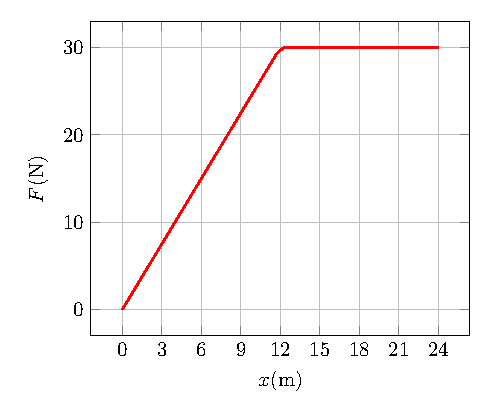
\includegraphics{hw-7-fig-1}
  \caption{Graph of the force $F$ with respect to distance.}
  \label{fig:hw-7-1}
\end{figure}
\end{problem}
\begin{proof}[Solution]
Remember that the work done by a force $F(x)$ over a distance
$a\leq x\leq b$ is given by the formula
\begin{equation}
  \label{eq:work}
W=\int_a^b F(x)\diff x.
\end{equation}
Since the graph in Figure (\ref{fig:hw-7-1}) is piecewise, all we need to
do is break up our interval $0\leq x\leq 24$ into the part where $y$ is a
diagonal line and where $y$ is a horizontal line, compute the work done on
each interval, $W_1$ and $W_2$, and add them up to get the total work
$W=W_1+W_2$.  First, note that over $0\leq x\leq 12$,
$F(x)=\frac{30}{12}x=\frac{5}{2}x$ so the work done from $0\leq x\leq 12$
is
\[
W_1=\int_0^{12}\frac{5}{2}x\diff x=
\left.\frac{5}{4}x^2\right|_0^{12}=
\frac{5}{4}(12)^2=\SI{180}{\joule}.
\]
Next, we see that $F(x)=30$ is constant for all $12\leq x\leq 24$
so we have
\[
W_2=\int_{12}^{24}F(x)\diff x=
\int_{12}^{24}30\diff x=
\left.30x\right|_{12}^{24}=
30\cdot 24-30\cdot 12=30\cdot 12=\SI{360}{\joule}.
\]
Hence, the total work done by $F(x)$ over $0\leq x\leq 24$ is
\[
  \boxed{W=W_1+W_2=\SI{180}{\joule}+\SI{360}{\joule}=\SI{540}{\joule}.}
\]
\end{proof}
\begin{problem}[WebAssign, HW8, 3]
A force of $6$ lb is required to hold a spring stretched $8$ in beyond its
natural length. How much work $W$ is done in stretching it from its natural
length to $14$ in beyond its natural length?
\end{problem}
\begin{proof}[Solution]
Recall \href{https://en.wikipedia.org/wiki/Hooke's_law}{Hooke's law} for
the force required to stretch a spring a distance $x$  beyond its natural
length
\begin{equation}
\label{eq:hookes-law}
F(x)=kx.
\end{equation}
Now, we are given a force of $6$ lb and a distance of $8$ in. Using this
information, we can figure out what the coefficient $k$ must be:
\[
k=F/x=6/8\mathrm{lb}/\mathrm{in}.
\]
Using the Equation (\ref{eq:work}) for work, we have that the work done on
a spring by stretching it from $x_1$ to $x_2$ is
\begin{equation}
\label{eq:work-on-spring}
W(x_1,x_2)=\int_{x_1}^{x_2}F(x)\diff x=\int_{x_1}^{x_2}kx\diff x=\left.\frac{1}{2}kx^2\right|_{x_1}^{x_2}=\frac{1}{2}k\left({x_1}^2-{x_2}^2\right)
\end{equation}
so, plugging in $14$, into our equation $W(x')$ above we get
\[
W(14)=\frac{1}{2}\cdot \frac{6}{8}\cdot
14^2=7\cdot\frac{6}{8}=\boxed{\frac{49}{8}\text{ ft-lb}.}
\]
\end{proof}
\begin{problem}[WebAssign, HW8, 4]
If the work required to stretch a spring $3$ ft beyond its natural length is
$9$ ft-lb, how much work is needed to stretch it $9$ in beyond its natural
length?
\end{problem}
\begin{proof}[Solution]
We employ the same idea as the one we used to calculate the work on the
last problem. First, we find the coefficient $k$, wit the help of Equation
(\ref{eq:work-on-spring}) this value will be
\[
k=\frac{2W}{x^2}=\frac{2\cdot 9}{9}=2\text{ lb}/\text{ft}.
\]
Now, convert our $9\text{ in}$ to ft we get $3/4\text{ ft}$. Lastly,
applying Equation (\ref{eq:work-on-spring}) on $3/4\text{ ft}$ we get
\[
W(3/4)=\frac{1}{2}\cdot 2\cdot (3/4)^2=\boxed{\frac{9}{16}\text{ in-lb}.}
\]
\end{proof}
\begin{problem}[WebAssign, HW8, 5]
An aquarium $\SI{6}{\meter}$ long, $\SI{1}{\meter}$ wide, and
$\SI{1}{\meter}$ deep is full of water. Find the work needed to pump half
of the water out of the aquarium. (Use $\SI{9.8}{\meter/\second^2}$ for $g$
and the fact that the density of water is
$\SI{1000}{\kilo\gram/\meter^3}$.)
\begin{itemize}
\item Show how to approximate the required work by a Riemann sum. (Let $x$
  be the height in meters below the top of the tank. Enter $x_i^*$ as $x_i$.)
\item Express the work as an integral.
\end{itemize}
\end{problem}
\begin{proof}[Solution]
Let's place the origin at the top of the tank. Then, the expression for the
work required to pump out half the water from our tank will be given
approximately by
\[
W(x)\approx\lim_{n\to\infty}\sum_{i=1}^n9.8\cdot1000\cdot 6\cdot x_i\Delta
x=\boxed{\sum_{i=1}^{n}58800 x_i^*\Delta x.}
\]
\\\\
Now we compute the integral from $0\leq x\leq 1/2$. We have
\[
W=58800\int_0^{1/2} x\diff x=5800\left(\left.\frac{1}{2}x^2\right|_0^{1/2} \right)=29400\left((1/2)^2-0\right)=\boxed{\SI{7350}{\joule}.}
\]
\end{proof}

\begin{problem}[WebAssign, HW8, 6]
A tank is full of water (see Figure \ref{fig:hw-7-2}). Find the work $W$
required to pump the water out of the spout. (Use
$\SI{9.8}{\meter/\second^2}$ for $g$. Use $\SI{1000}{\kilo\gram/\meter^3}$
as the weight density  of water. Assume that $a=\SI{4}{\meter}$,
$b=\SI{4}{\meter}$, $c=\SI{12}{\meter}$, and $d=\SI{2}{\meter}$.)
\begin{figure}[htbp]
  \centering
  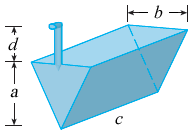
\includegraphics[scale=0.45]{hw-7-fig-2}
  \caption{A sketch of the tank.}
  \label{fig:hw-7-2}
\end{figure}
\end{problem}
\begin{proof}[Solution]
The work required to pump the water out of the spout of a tank with the
dimensions above is given by the
\[
W=\lim_{n\to\infty}\sum_{i=0}^n F(x_i)\Delta x
\]
where $\SI{0}{\meter}\leq x\leq\SI{8}{\meter}$. Now, the first thing we
need to do is to find the way the force changes as we move up the tank. Let
$x$ be the vertical distance from the bottom of the tank and $y$ be the
horizontal distance from. Then, the work needed to lift the slice slice of
volume $\Delta V$ that is a distance $(4+2)-x$ from the spout is
\begin{equation}
\label{eq:weight-density}
W(x)\approx g\rho(6-x)\Delta V,
\end{equation}
where $\rho$ is the density of the water and $g$ is gravity. Now, how does
our little slice of volume change as we move up the tank? If $y$ is the
side of the right-triangle made by going up a distance $x$ up the tank, then
\[
\frac{x}{y}=\frac{4}{4}=1
\]
since the triangles are similar. Hence, $y=2x$ so the volume change will be
\[
V(x)\approx 12\cdot\frac{1}{2}(2x)\Delta x=12x\Delta x(6-x),
\]
this is just the area of a triangle $x\Delta x$ (base times height) times
the depth $\SI{12}{\meter}$. Hence, the, plugging in the last equation into
our equation for the force (Equation (\ref{eq:weight-density})) will be
\[
W(x)\approx g\rho(6-x)\left(12 x\Delta x\right)=117600(6-x)x\Delta x
\]
Last but not least, we compute the limit as
$n\to\infty$,
\begin{align*}
W&=\lim_{n\to\infty}\sum_{i=0}^n W(x_i)\Delta x\\
\shortintertext{this is just the integral}
 &=117600\int_0^4(6-x)x\diff x\\
 &=117600\int_0^46x-x^2\diff x\\
 &=117600\left(\left.3x^2-\frac{1}{3}x^3\right|_0^4\right)\\
 &=117600\left(3\cdot 4^2-\frac{4^3}{3}-(0-0)\right)\\
 &=117600\left(\frac{3\cdot 3\cdot 4^2-4^3}{3}\right)\\
 &=117600\left(4^2\cdot\frac{9-4}{3}\right)\\
 &=117600\left(4^2\cdot\frac{5}{3}\right)\\
 &=\boxed{\SI{3136000}{\joule}.}
\end{align*}
\end{proof}
% p453:11,14
\begin{problem}[WebAssign, HW8, 7]
Consider the given function and the given interval
\[
f(x)=10\sin x-5\sin 2x,\quad[0,\pi]
\]
\begin{enumerate}[label=(\alph*)]
\item Find the average value $f_{\text{ave}}$ of $f$ on the given
  interval.
\item Find $c$ such that $f_{\text{ave}}=f(c)$.
\item Sketch the graph of $f$ and a rectangle whose area is the same as the
  area under the graph of $f$.
\end{enumerate}
\end{problem}
\begin{proof}[Solution]
(a) Recall the definition of the average of a function over an interval
$[a,b]$, it is
\begin{equation}
  \label{eq:average}
f_{\text{ave}}=\frac{1}{b-a}\int_a^b f\diff x.
\end{equation}
Now, all we need to do is calculate the integral of our $f$ and divide that
value by $\pi-0$, i.e.,
\begingroup
\allowdisplaybreaks
\begin{align*}
f_{\text{ave}}&=\frac{1}{\pi}\int_0^\pi f(x)\diff x\\
&=\frac{1}{\pi}\int_0^\pi 10\sin x-5\sin 2x\diff x\\
&=\frac{1}{\pi}\left(\left.-10\cos x+\frac{5}{2}\cos
  2x\right|_0^\pi\right)\\
&=\frac{1}{\pi}\left(-10\cos\pi+\frac{5}{2}\cos 2\pi-\left(-10\cos
  0+\frac{5}{2}\cos 0\right)\right)\\
&=\frac{1}{\pi}\left(10+\frac{5}{2}+10-\frac{5}{2}\right)\\
&=\frac{1}{\pi}\cdot 20\\
&=\boxed{\frac{20}{\pi}.}
\end{align*}
\endgroup
\\\\
(b) For this part all we need to do is set the equation $f(x)=10\sin
x-5\sin 2x$ equal to $20/\pi$ and solve for $x$:
\[
10\sin x-5\sin 2x=5(2\sin x-\sin 2x)=\frac{20}{\pi}
\]
so
\[
  2\sin x-\sin 2x=\frac{4}{\pi}.
\]
I can't think of any way to solve this than plugging it into your
calculator and having your calculator approximate the solution (your
calculator probably uses
\href{https://en.wikipedia.org/wiki/Newton's_method}{Newton's method},
which you will learn about later in your career). The values are about
\ul{$c\approx 1.238$ and $2.808$.}
\\\\
(c) Sketching the graph is easy and the box having the same area as will
have height equal to $20/\pi$ and length $\pi$. Multiply these together and
we get the area under the curve, which we computed to be $20$.
\end{proof}
\begin{problem}[WebAssign, HW8, 8]
Find the numbers b such that the average value of
$f(x)=7+10x-9x^2$ on the interval $[0,b]$ is equal to $8$.
\end{problem}
\begin{proof}[Solution]
This exercise is easy-peasy :-). All you need to do is compute the average
\[
f_\text{ave}=\frac{1}{b-0}\int_0^b7+10x-9x^2\diff x=7+5b-3b^2.
\]
Now, set the above equal to $8$ and we have
\[
7+5b-3b^2=8
\]
and solve for $b$. We get \ul{$b=(5-\sqrt{13})/6$ or $(5+\sqrt{13})/6$.}
\end{proof}

%%% Local Variables:
%%% mode: latex
%%% TeX-master: "../MA166-HW-Current"
%%% End:
